\documentclass[12pt,  a4paper, ngerman]{article}
\usepackage[a4paper, total={6in, 8in}, margin=1.1in]{geometry}
\usepackage[default,scale=0.95]{opensans}
\usepackage[section]{minted}
\usepackage{mdframed}
\usepackage{lingmacros}
\usepackage{tree-dvips}
\usepackage{listings}
\usepackage{blindtext}
\usepackage{amsmath}
\usepackage{hyperref}
\usepackage{graphicx}
\graphicspath{ {./images/} }


\renewcommand\seriesdefault{l}
\renewcommand\mddefault{l}
\renewcommand\bfdefault{sb}
\renewcommand{\contentsname}{Inhalt}
\renewcommand{\refname}{Literaturverzeichnis}

\hypersetup{
    colorlinks=true,
    linkcolor=black,
    filecolor=magenta,      
    urlcolor=cyan,
    citecolor=cyan
}

\title{Semesterarbeit Teil 1: Rekursion mit Python anhand der Fibonacci-Folge}
\date{Februar, 2020}
\author{Patrick Michel\\
FFHS - Fernfachhochschule Schweiz\\
6. Semester AnPy\thanks{AnPy, Analysis mit Python, BSc INF 2017 Pas, BE1-I, FS20, Geuss Markus}
}

\begin{document}

\definecolor{bg}{rgb}{0.95,0.95,0.95}

\begin{titlepage}

\maketitle
\tableofcontents

\end{titlepage}

\section{Einleitung}
Die folgende Arbeit befasst sich mit der Fibonacci-Folge. 
Dabei handelt es sich um eine unendliche Reihe von natürlichen Zahlen.
Die Folge ist benannt nach Leonardo Fibonacci, 
der damit im 1300 Jahrhunder das Wachstum einer Kaninchenpopulation zu beschreiben versuchte.
Heute wird die Zahlenfolge in einer abgewandelter Form zum Beispiel auch
in der agilen Welt zur Schätzung von Arbeitsaufwänden verwendet (Story Points).
Die Zahlenfolge beginnt üblicherweise mit einer 0.
Darauf folgend zwei mal die 1 und danach wird die Folge nachvollziehbar.
Nachfolgend zur Nachvollziehbarkeit die definition der ersten 5 Folgen:
\begin{equation}
  f_0 := 0,
  f_1 := 1,
  f_2 := 1,
  f_3 := 2,
  f_4 := 3
\end{equation}
Daraus ergibt sich folgende allgemeine Definition:
\begin{equation}
  f_n := f_{n-1} + f_{n-2} \text{ für } n \ge 2
\end{equation}
Auf Basis dieser Definition sollen nun folgende Aufgaben
erledigt werden:
\begin{enumerate}
  \item Implementieren Sie eine Python-Funktion \textit{fib(n)}, die die n-te Fibonacci-Zahl bestimmt.
  \item Eine naive Implementierung setzt die obige Rekursionsgleichung direkt um. Schreiben Sie eine weitere Python-Funktion, die berechnet, wie viele Funktionsaufrufe on fib notwendig sind, um die n-te Fibonacci-Zahl zu berechnen.
  \item Vergleichen Sie die Anzahl der Funktionsaufrufe von fib zur Bestimmung einer Fibonacci-Zahl mit den Fibonacci-Zahlen selber. Können Sie eine Vermutung aufstellen?
  \item Verwenden Sie die Funktion \textit{time()} aus dem Modul time, um zu bestimmen, wie lange die Funktion fib benötigt, um eine Fibonacci-Zahl zu bestimmen.
  \item Implementieren Sie eine weitere Python-Funktion zur Berechnung der n-ten Fibonacci-Zahl, die möglichst effizient ist. (Hinweis: das kann rekursiv oder iterativ gelöst werden.)
\end{enumerate}
\subsection{Abstract}

\newpage

\section{Naive Implementierung}
Im folgenden beschäftigen wir uns mit einer naiven
Implementierung der Fibonacci-Folge mit Python.
Diese soll wie auch die mathematische Definition rekursiv geschrieben werden.
\subsection{Der Algorithmus}
Als Editor wird VS Code mit dem Python Plugin verwendet.
Die Schwierigkeit der Implementierung besteht in den
ersten 2 Folgen da diese noch nicht der üblichen Logik folgen.
Daher ist für diese zwei Werte eine Grenzfallbehandlung
zu Implementieren. Dies wurde mithilfe einer \textit{if-else}
Anweisung in der Rückgabeanweisung umgesetzt:
\begin{mdframed}[backgroundcolor=bg]
    \inputminted{Python}{src/naive_fibonacci.py}
\end{mdframed}
Beim Aufruf der Funktion kommen folgende Outputs zustande:
\begin{mdframed}[backgroundcolor=bg]
    \inputminted{Python}{src/naive_fibonacci_test.py}
\end{mdframed}
Durch die oben durchgeführten \textit{print} Tests konnte
zudem die maximale Rekursionstiefe, die Python standardmässig
gesetzt hat, ermittelt werden. 
Diese liegt bei 1000. 
Weiter kann durch die Analyse des Codes folgende
Laufzeit des Algorithmus definiert werden:
\begin{equation}
    \mathcal{O}(n + 1)
\end{equation}



\newpage

\section{Rekursionstiefe analysieren}
Der folgende Abschnitt beschäftigt sich mit der Rekursionstiefe
der zuvor beschriebenen Implementation. 
Im folgenden beschäftigen wir uns mit einer naiven
Implementierung der Fibonacci-Folge mit Python.
Diese soll wie auch die mathematische Definition rekursiv geschrieben werden.
Als Editor wird VS Code mit Python Plugin verwendet.
Die Schwierigkeit der Implementierung besteht in den
ersten 2 Folgen da diese noch nicht der üblichen Logik folgen.
Daher ist für diese zwei Werte eine Grenzfallbehandlung
zu Implementieren. Dies wurde mithilfe einer \textit{if-else}
Anweisung in der Rückgabeanweisung umgesetzt:
\begin{mdframed}[backgroundcolor=bg]
    \inputminted{Python}{src/count_fibonacci.py}
\end{mdframed}
Beim Aufruf der Funktion kommen folgende Outputs zustande:
\begin{mdframed}[backgroundcolor=bg]
    \inputminted{Python}{src/count_fibonacci_test.py}
\end{mdframed}
Durch die oben durchgeführten \textit{print} Tests konnte
zudem die maximale Rekursionstiefe, die Python standardmässig
gesetzt hat, ermittelt werden. 
Diese liegt bei 1000. 
Wir werden diese Implementierung nun
auf verschiedene Arten analysieren um mehr über das 
Verhalten der Funktion beim Aufruf zu erfahren.



\newpage

\subsection{Rekursionstiefe und Fibonacci-Folge im Vergleich}
Der folgende Abschnitt beschäftigt sich mit der Rekursionstiefe
der zuvor beschriebenen Implementation. Das bedeutet die
folgende Implementation ermöglicht es herauszufinden wieviele
gestapelte rekursive Aufrufe die naive Implementation machen
muss um eine bestimmte Fibonacci Zahl zu berechnen.
\begin{mdframed}[backgroundcolor=bg]
    \inputminted{Python}{src/count_fibonacci.py}
\end{mdframed}
Beim Aufruf der Funktion kommen folgende Outputs zustande:
\begin{mdframed}[backgroundcolor=bg]
    \inputminted{Python}{src/count_fibonacci_test.py}
\end{mdframed}
Was auf den ersten Blick auffällt ist das geringe Wachstum 
der rekursiven Aufrufe im Vergleich zu den hohen Fibonacci-Folgen
welche daraus generiert werden kann. Die obige Implementation
zur Ermittlung der Rekursiontiefe gehört zu folgender 
Gruppe der Laufzeitkomplexität:
\begin{equation}
    \mathcal{O}(n^2 + 1)
\end{equation}

\newpage
\section{Optimierung der Funktion}
Der folgende Abschnitt beschäftigt sich mit der 
Optimierung der zuvor beschriebenen rekursiven
Implementation. Dafür wurden zwei Optimierungen vorgenommen.
Die erste Optimierung ist eine Cachliste welche alle bereits
berechneten Resultate zwischenspeichert. Eine weitere
Optimierung ist eine iterative Implementation.
Dadurch können viel höhere Finonacci Zahlen berechnet werden
und diese stossen nie auf eine Funktionsaufruflimitte.
Auch wird dadurch viel weniger Overhead auf dem Stack generiert:
\begin{mdframed}[backgroundcolor=bg]
    \inputminted{Python}{src/advanced_fibonacci.py}
\end{mdframed}

\newpage

Beim Aufruf der Funktion kommen folgende Outputs zustande:
\begin{mdframed}[backgroundcolor=bg]
    \inputminted{Python}{src/advanced_fibonacci_test.py}
\end{mdframed}
Was nun beim Test auffällt ist bei der 999. Fibonacci-Zahl
kommt kein Fehler mehr. Und wenn nun die Funktion mehrfach
für die gleiche Fibonacci-Zahl aufgerufen wird,
kommt das Resultat ohne grosse Berechnung direkt aus dem
Cache mit einer Laufzeitkomplexität von:
\begin{equation}
    \mathcal{O}(n)
\end{equation}

\newpage
\section{Resultate und Vergleich}
In diesem Abschnitt geht es nun um die eriehlten Resultate und
einem Vergleich zwischen der rekursiven und iterativen
Implementation. Um einen solchen Vergleich zu ermöglichen habe
ich folgende Funktionen zum Berechnen der Laufzeit implementiert.
Die Perioden definieren wieviel mal die Finonacci-Zahl
berechnet wird und daraus wird dann der Mittelwert genommen.
So werden stark abweichende Messungen verhindert:

\begin{mdframed}[backgroundcolor=bg]
    \inputminted{Python}{src/time_fibonacci.py}
\end{mdframed}

\newpage

Um einen einfacheren Vergleich zu ermöglichen habe ich
für die definition der Tests die matplotlib verwendet.
Diese ermöglicht es einfach aus Zahlen ein visuelles
Diagramm zu erstellen. Die Implementation des Vergleichs
sieht folgendermassen aus:

\begin{mdframed}[backgroundcolor=bg]
    \inputminted{Python}{src/time_fibonacci_test.py}
\end{mdframed}

Wie nachfolgende ganz deutlich aus den Diagrammen herauszulesen ist,
ist die iterative Implementation definitiv mit Abstand performanter.
Bei der 3000. Fibonacci-Zahl ergibt sich eine 5x bessere
Performance. Und würde dann noch die Caching Funktionalität
der optimierten Version zum tragen kommen, wäre der
Performancegewinn noch einmal deutlich grösser.

\begin{figure}[h]
    \centering
    \caption{Die rekursive Implementation}
    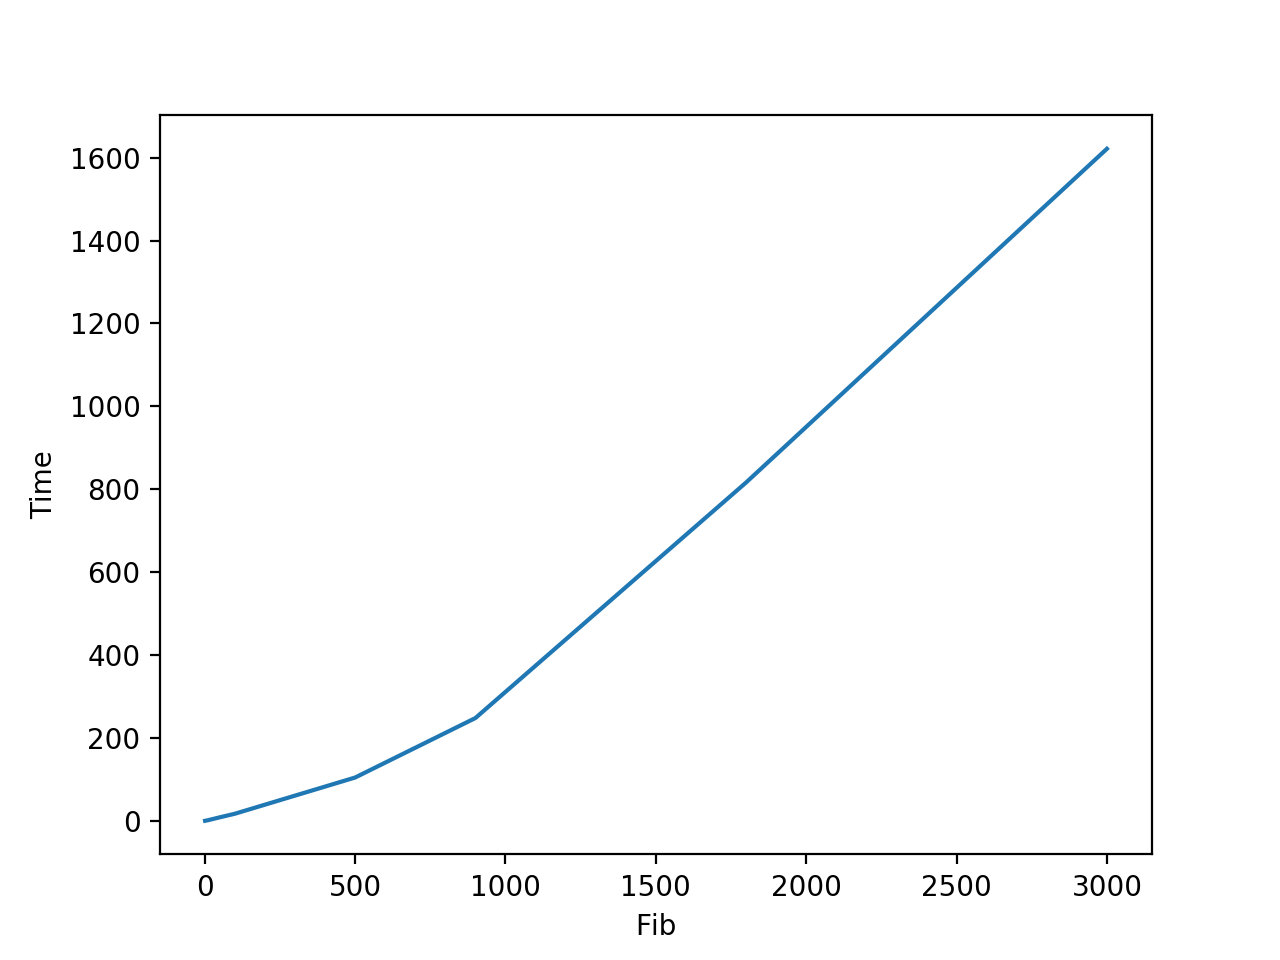
\includegraphics[width=0.8\textwidth]{Figure_1}
    \caption{Die iterative Implementation}   
    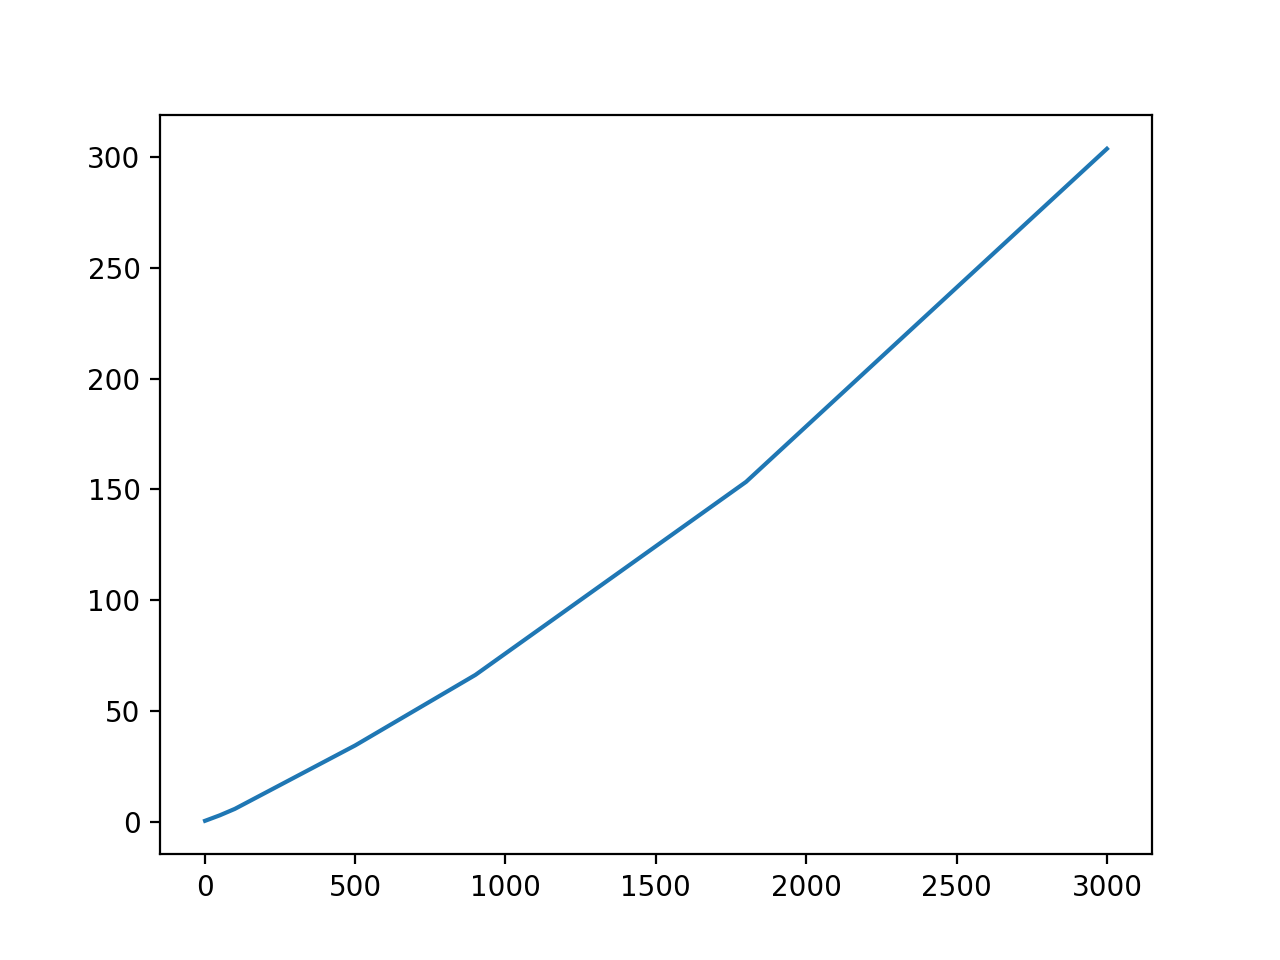
\includegraphics[width=0.8\textwidth]{Figure_2}
\end{figure}

\section{Quellen}

\begin{thebibliography}{quellen}
         
    \bibitem{python_max_rec} 
    Python maximales Rekursionslimit,\\
    \texttt{\url{https://stackoverflow.com/questions/3323001/what-is-the-maximum-recursion-depth-in-python-and-how-to-increase-it}},\\
    05.02.2020
    \end{thebibliography}


\end{document}